\documentclass[aspectratio=169, table]{beamer}

\usepackage{array}
\usepackage{colortbl}
\usepackage{tabularx}
\usepackage{xcolor}
\usepackage{tikz}
\usetikzlibrary{arrows.meta, positioning, calc, fit}

\makeatletter
\def\input@path{{../theme/}}
\makeatother
\graphicspath{{../theme/}{../../figures/}}
\usetheme{Pradita}

\newcommand{\sectionframe}[1]{%
  \begin{frame}{\hfill}
    \centering
    \Huge{\textbf{#1}}
  \end{frame}
}

\newcommand{\takeaway}[1]{%
  \vspace{4pt}
  {\footnotesize #1}
}

\title{\huge Lapisan Data\\
  \vspace{8pt}
  pada ArchiMate}
\subtitle{IT30713 - Enterprise \& Platform Architecture}
\author{\textbf{Alfa Yohannis}}
\date{27 Juni 2026}

\begin{document}

\frame{\titlepage}

\begin{frame}[fragile]
  \frametitle{Contents}
  \vspace{20pt}
  \begin{columns}[t]
    \column{0.5\textwidth}
    \tableofcontents[sections={1-4}]

    \column{0.5\textwidth}
    \tableofcontents[sections={5-8}]
  \end{columns}
\end{frame}

\begin{frame}{\hfill}
  \centering
  \Huge{\textbf{Bisnis sudah dipetakan---data apa yang mengalir di dalamnya?}}
\end{frame}

% ============================================================
\section{Orientasi Bab}
\sectionframe{Orientasi Bab}

\begin{frame}{Tujuan Pembelajaran}
  \vspace{6pt}
  \begin{itemize}
    \item Menjelaskan elemen informasi ArchiMate: \textbf{objek bisnis}
          (konseptual), \textbf{objek data} (logis), dan \textbf{representasi}.
    \item Menyusun \textbf{model data} konseptual/logis dan memetakan objek data
          ke \textbf{proses} yang mengaksesnya.
    \item Menempatkan analisis dalam \textbf{TOGAF ADM Fase C (Data)}: arsitektur
          data \emph{baseline}, \emph{target}, dan kesenjangan.
    \item Mengaitkan rancangan data dengan \textbf{tata kelola} dan
          \textbf{perlindungan data pribadi} (UU PDP, PP 71, SNAP BI, Satu Data).
  \end{itemize}
  \takeaway{Arah sesi: dari ``bagaimana bisnis bekerja'' menuju ``data apa yang
  mengalir dan aturan mainnya''.}
\end{frame}

\begin{frame}{Ringkasan Awal Bab}
  \vspace{6pt}
  \begin{itemize}
    \item Dalam ArchiMate, data adalah bagian \textbf{lapisan aplikasi}:
          \emph{data object} = struktur pasifnya.
    \item Prinsip kunci: \textbf{objek data diturunkan dari objek bisnis}
          (relasi \emph{realisasi}).
    \item Studi kasus berjalan: entitas data rel \textbf{API Transfer Dana}---dari
          Instruksi Transfer sampai Catatan Rekonsiliasi.
    \item Keluaran bab memperkuat \textbf{Metode} \& \textbf{Analisis} makalah:
          model data \& matriks data-ke-proses.
  \end{itemize}
  \takeaway{Banyak masalah transformasi sebenarnya masalah data: definisi,
  kepemilikan, kualitas, dan privasi.}
\end{frame}

% ============================================================
\section{Mengapa Lapisan Data}
\sectionframe{Mengapa Lapisan Data}

\begin{frame}{Posisi Lapisan Data dalam ArchiMate}
  \vspace{2pt}
  \centering
  \scalebox{0.74}{
    \begin{tikzpicture}[
      font=\small\bfseries,
      node distance=2.2mm,
      layer/.style={draw, rounded corners=1.5mm, align=left, minimum width=82mm,
        minimum height=10mm, inner xsep=4mm},
      strat/.style={layer, fill=orange!16},
      biz/.style={layer, fill=praditagreen!22},
      app/.style={layer, fill=blue!24, draw=blue!70!black, line width=0.5mm},
      tech/.style={layer, fill=gray!18},
      impl/.style={layer, fill=orange!10},
    ]
      \node[strat] (s) {STRATEGI\\
        \footnotesize\mdseries Sumber daya, kapabilitas, arah tindakan};
      \node[biz, below=of s] (b) {BISNIS\\
        \footnotesize\mdseries Aktor, peran, proses, layanan, \textbf{objek bisnis}};
      \node[app, below=of b] (a) {APLIKASI \quad$\leftarrow$ \emph{fokus: DATA}\\
        \footnotesize\mdseries Komponen, layanan, antarmuka, \textbf{objek data}};
      \node[tech, below=of a] (t) {TEKNOLOGI (\& FISIK)\\
        \footnotesize\mdseries Node, perangkat, jaringan, \emph{artifact}};
      \node[impl, below=of t] (i) {IMPLEMENTASI \& MIGRASI\\
        \footnotesize\mdseries \emph{Work package}, \emph{deliverable}, \emph{gap}};
      \node[draw, rounded corners=2mm, fill=purple!22, align=center,
        text width=16mm, minimum height=60mm, right=5mm of a, font=\bfseries]
        (mot) {M\\O\\T\\I\\V\\A\\S\\I\\[2mm]\footnotesize\mdseries (mengapa)};
    \end{tikzpicture}
  }

  \takeaway{\emph{Objek data} menempati struktur pasif lapisan aplikasi;
  dipetakan ke fase \textbf{C (Arsitektur Sistem Informasi)} TOGAF ADM.}
\end{frame}

\begin{frame}{Data: Konseptual $\rightarrow$ Logis $\rightarrow$ Perwujudan}
  \vspace{4pt}
  \centering
  \scalebox{0.9}{
    \begin{tikzpicture}[
      font=\footnotesize,
      lvl/.style={rectangle, rounded corners=1.5mm, thick, align=center,
        minimum height=11mm, text width=40mm},
      konsep/.style={lvl, draw=praditagreen, fill=praditagreen!14},
      logis/.style={lvl, draw=blue!70!black, fill=blue!12},
      fisik/.style={lvl, draw=gray!60, fill=gray!14},
      link/.style={-Latex, thick, draw=gray!60}
    ]
      \node[konsep] (k) {\textbf{Konseptual}\\{\scriptsize Business Object}};
      \node[logis, below=7mm of k] (l) {\textbf{Logis}\\{\scriptsize Data Object}};
      \node[fisik, below=7mm of l] (f) {\textbf{Fisik}\\{\scriptsize Artifact (Bab 7)}};
      \draw[link] (l) -- node[right]{\scriptsize merealisasikan} (k);
      \draw[link] (f) -- node[right]{\scriptsize merealisasikan} (l);
      \node[align=left, text width=46mm, right=7mm of k] {\scriptsize Entitas informasi \& relasi};
      \node[align=left, text width=46mm, right=7mm of l] {\scriptsize Atribut, struktur, kunci};
      \node[align=left, text width=46mm, right=7mm of f] {\scriptsize Tabel, berkas pada teknologi};
    \end{tikzpicture}
  }

  \takeaway{Objek data \emph{diturunkan dari} objek bisnis; bab ini fokus pada dua
  tingkat teratas (konseptual \& logis).}
\end{frame}

% ============================================================
\section{TOGAF ADM Fase C}
\sectionframe{TOGAF ADM Fase C:\\ Arsitektur Data}

\begin{frame}{Siklus TOGAF ADM}
  \vspace{8pt}
  \begin{columns}[c]
    \column{0.4\textwidth}
    \centering
    \scalebox{0.85}{
      \begin{tikzpicture}[
        font=\footnotesize\bfseries,
        phase/.style={circle, draw=praditagreen, line width=0.4mm,
          fill=praditagreen!15, minimum size=11mm, inner sep=0pt},
        reqman/.style={circle, draw=blueColor, line width=0.4mm, fill=blueColor!15,
          minimum size=21mm, inner sep=1pt, align=center, font=\scriptsize\bfseries},
        prelim/.style={circle, draw=orange!80!black, line width=0.4mm,
          fill=orange!25, minimum size=13mm, inner sep=0pt, align=center,
          font=\scriptsize\bfseries},
        ring/.style={-Latex, draw=praditagreen!75, line width=0.4mm},
        spoke/.style={draw=blueColor!35, line width=0.25mm},
      ]
        \node[reqman] (rm) at (0,0) {Manajemen\\Requirements};
        \foreach \ang/\lab in {90/A, 45/B, 0/C, -45/D, -90/E, -135/F, 180/G, 135/H}
          \node[phase] (\lab) at (\ang:2.6cm) {\lab};
        \node[prelim] (P) at (90:4.1cm) {Prelim.};
        \foreach \lab in {A,B,C,D,E,F,G,H} \draw[spoke] (\lab) -- (rm);
        \foreach \a/\b in {A/B, B/C, C/D, D/E, E/F, F/G, G/H, H/A}
          \draw[ring] (\a) to[bend left=12] (\b);
        \draw[ring, draw=orange!80!black] (P) -- (A);
        \node[phase, fill=blue!45, line width=0.7mm] at (0:2.6cm) {C};
      \end{tikzpicture}
    }
    \column{0.6\textwidth}
    {\footnotesize TOGAF (\emph{The Open Group Architecture Framework}); ADM
    (\emph{Architecture Development Method})---metode pengembangan arsitektur
    dengan siklus berulang.\par}
    \vspace{5pt}
    \footnotesize
    \begin{itemize}\setlength{\itemsep}{1.0pt}
      \item \textbf{Prelim.}---Persiapan \& prinsip
      \item \textbf{A}---Visi Arsitektur
      \item \textbf{B}---Arsitektur Bisnis
      \item \textbf{\textcolor{blue!70!black}{C---Arsitektur Sistem Informasi
            (Data \& Aplikasi)}} $\leftarrow$ \emph{fokus sesi ini (Data)}
      \item \textbf{D}---Arsitektur Teknologi
      \item \textbf{E}---Peluang \& Solusi
      \item \textbf{F}---Perencanaan Migrasi
      \item \textbf{G}---Tata Kelola Implementasi
      \item \textbf{H}---Manajemen Perubahan Arsitektur
      \item \textbf{Manajemen Requirements}---di pusat, menyetir semua fase
    \end{itemize}
  \end{columns}
\end{frame}

\begin{frame}{Fase C (Data): Lima Langkah}
  \vspace{2pt}
  \footnotesize
  \begin{columns}[t]
    \column{0.5\textwidth}
    \textbf{Apa \& Mengapa}
    \begin{itemize}\setlength{\itemsep}{2.5pt}
      \item Fase C menerjemahkan arsitektur bisnis menjadi \emph{sistem
            informasi}: data lalu aplikasi.
      \item Sisi \textbf{Data}: entitas, model data, dan pemetaan ke proses.
      \item Menghasilkan \emph{baseline}, \emph{target}, dan analisis
            \textbf{kesenjangan}.
    \end{itemize}
    \column{0.5\textwidth}
    \textbf{Lima Langkah}
    \begin{enumerate}\setlength{\itemsep}{2.5pt}
      \item Ruang lingkup \& prinsip data.
      \item Arsitektur data \textbf{baseline}.
      \item Arsitektur data \textbf{target}.
      \item Analisis \textbf{kesenjangan}.
      \item Masukan ke sisi Aplikasi \& Fase D.
    \end{enumerate}
  \end{columns}
  \vspace{2pt}
  \takeaway{Keluaran: katalog entitas data, diagram model data, dan matriks
  data-ke-proses.}
\end{frame}

\begin{frame}{Baseline $\rightarrow$ Target Data (Bank Wanua)}
  \vspace{2pt}
  \scriptsize
  \setlength{\extrarowheight}{2pt}
  \arrayrulecolor{black!65}\setlength{\arrayrulewidth}{0.4pt}
  \begin{tabularx}{\textwidth}{|p{0.26\textwidth}|X|}
    \hline
    \rowcolor{blue!14}
    \textbf{Langkah Fase C (Data)} & \textbf{Artefak pada kasus Bank Wanua} \\
    \hline
    Ruang lingkup \& prinsip & Data transfer; data sebagai aset, minimisasi data pribadi, jejak audit melekat. \\
    \hline
    Baseline & Definisi rekening/limit/status beda antarkanal; catatan transaksi tanpa kunci seragam. \\
    \hline
    Target & Objek data mewujudkan objek bisnis; kunci transaksi seragam; audit \& hasil AML terstruktur. \\
    \hline
    Analisis kesenjangan & Entitas yang perlu distandardisasi, disatukan, atau dibangun kualitasnya. \\
    \hline
    Masukan berikutnya & Layanan data, komponen integrasi, mesin rekonsiliasi (lapisan aplikasi). \\
    \hline
  \end{tabularx}
  \vspace{4pt}
  \takeaway{Kesenjangan baseline--target data menjelaskan mengapa rekonsiliasi
  otomatis gagal pada kondisi kini.}
\end{frame}

\begin{frame}{}
  \centering
  \vspace{1mm}
  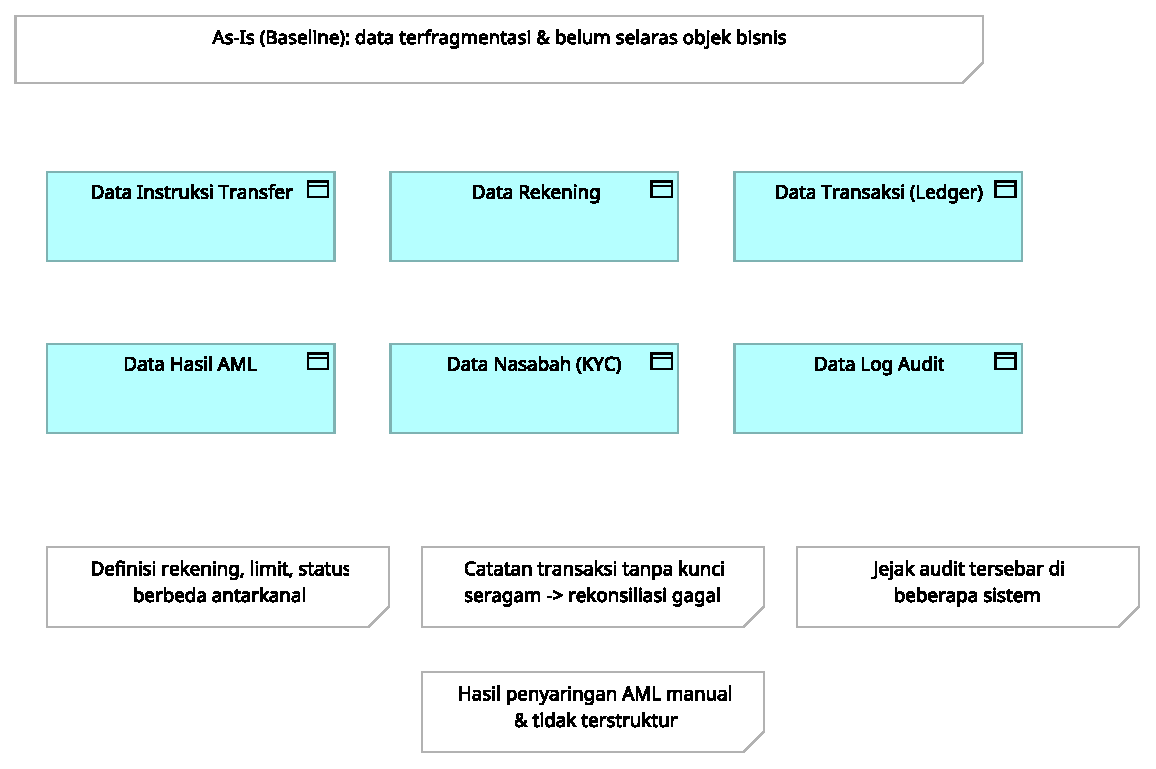
\includegraphics[width=\textwidth,height=.8\textheight,keepaspectratio]{data-asis.pdf}\\
  {\scriptsize \textbf{As-Is (Baseline):} data terfragmentasi; definisi berbeda
  antarkanal; catatan transaksi tanpa kunci seragam; audit tersebar.}
\end{frame}

\begin{frame}{}
  \centering
  \vspace{1mm}
  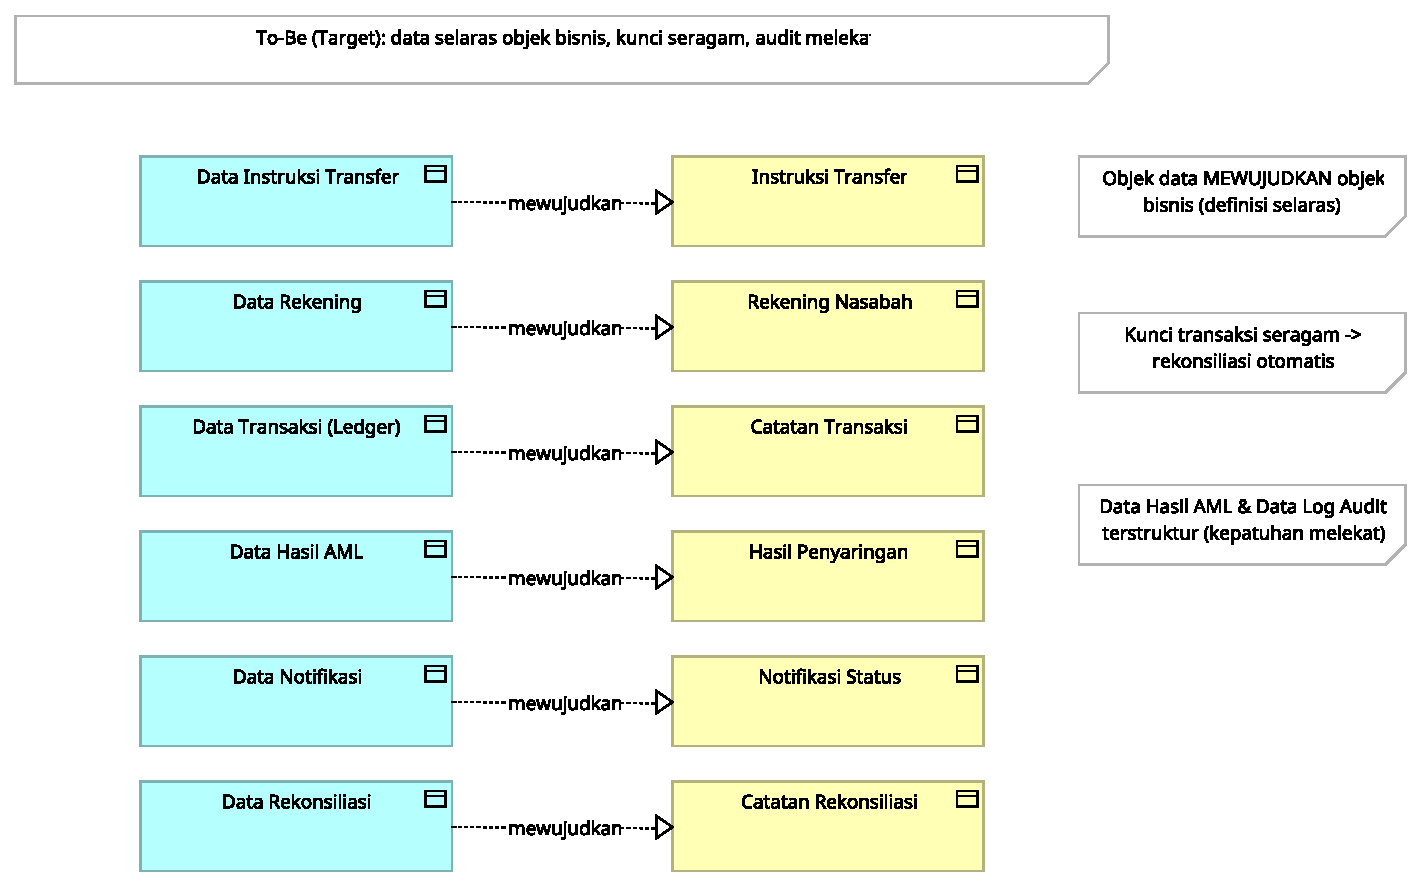
\includegraphics[width=\textwidth,height=.8\textheight,keepaspectratio]{data-tobe.pdf}\\
  {\scriptsize \textbf{To-Be (Target):} objek data \emph{mewujudkan} objek bisnis;
  kunci transaksi seragam; jejak audit \& hasil AML terstruktur.}
\end{frame}

% ============================================================
\section{Elemen Lapisan Data}
\sectionframe{Elemen Lapisan Data}

\begin{frame}{Tiga Notasi Informasi dan Simbolnya}
  \vspace{6pt}
  \begin{columns}[c]
    \column{0.55\textwidth}
    \centering
    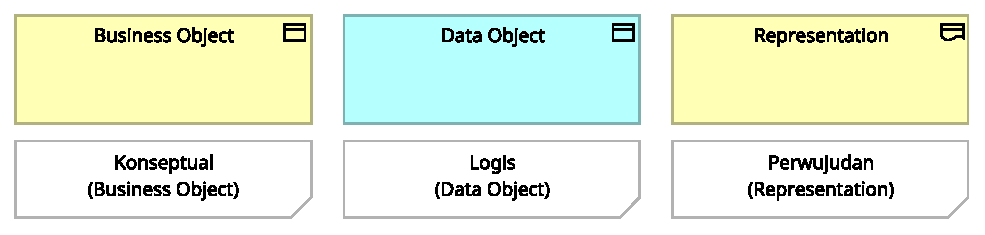
\includegraphics[width=\linewidth]{data-legend.pdf}
    \column{0.45\textwidth}
    \footnotesize
    \begin{itemize}\setlength{\itemsep}{4pt}
      \item \textbf{Business Object} -- konseptual: ``apa'' informasi bisnis.
      \item \textbf{Data Object} -- logis: bagaimana data disusun \& diproses;
            \emph{mewujudkan} objek bisnis.
      \item \textbf{Representation} -- perwujudan (struk, laporan, layar).
    \end{itemize}
  \end{columns}
  \takeaway{Konseptual $\rightarrow$ logis $\rightarrow$ perwujudan; objek data
  berwarna kebiruan (lapisan aplikasi).}
\end{frame}

\begin{frame}{Membedakan Elemen Informasi}
  \vspace{6pt}
  \begin{itemize}
    \item \textbf{Objek bisnis (business object):} informasi konseptual---
          ``Instruksi Transfer'', ``Rekening Nasabah''.
    \item \textbf{Objek data (data object):} representasi logis yang diproses
          aplikasi---``Data Instruksi Transfer''; \emph{mewujudkan} objek bisnis.
    \item \textbf{Representasi:} perwujudan yang dapat dipersepsi---``Struk
          Pembayaran''.
    \item \textbf{Relasi akses:} proses \emph{membaca}/\emph{menulis} objek
          \textbf{bisnis}; objek data merealisasikan objek bisnis itu.
  \end{itemize}
  \takeaway{Data \emph{diturunkan dari} objek bisnis; proses mengakses objek
  bisnis, bukan objek data secara langsung.}
\end{frame}

\begin{frame}{}
  \centering
  \vspace{1mm}
  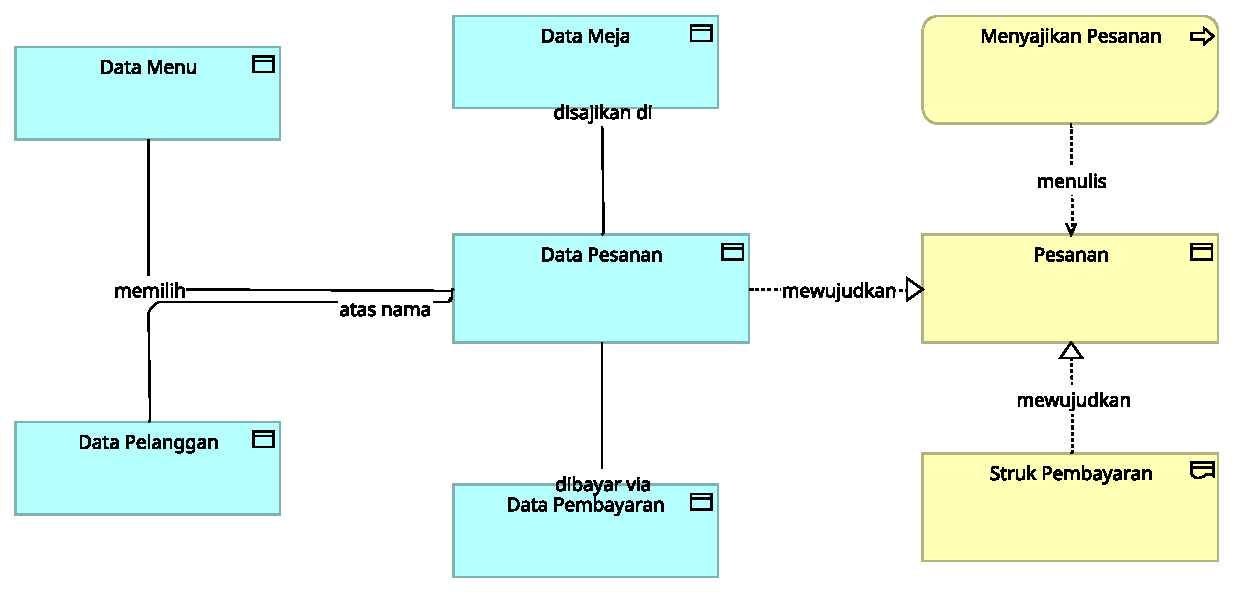
\includegraphics[width=\textwidth,height=.8\textheight,keepaspectratio]{data-contoh.pdf}\\
  {\scriptsize Contoh interaksi antar-elemen data (kasus restoran cepat saji):
  Data Pesanan mewujudkan Pesanan, diakses proses, diwujudkan sebagai Struk.}
\end{frame}

% ============================================================
\section{Studi Kasus: Model Data di Archi}
\sectionframe{Studi Kasus:\\ Arsitektur Data Transfer di Archi}

\begin{frame}{}
  \centering
  \vspace{1mm}
  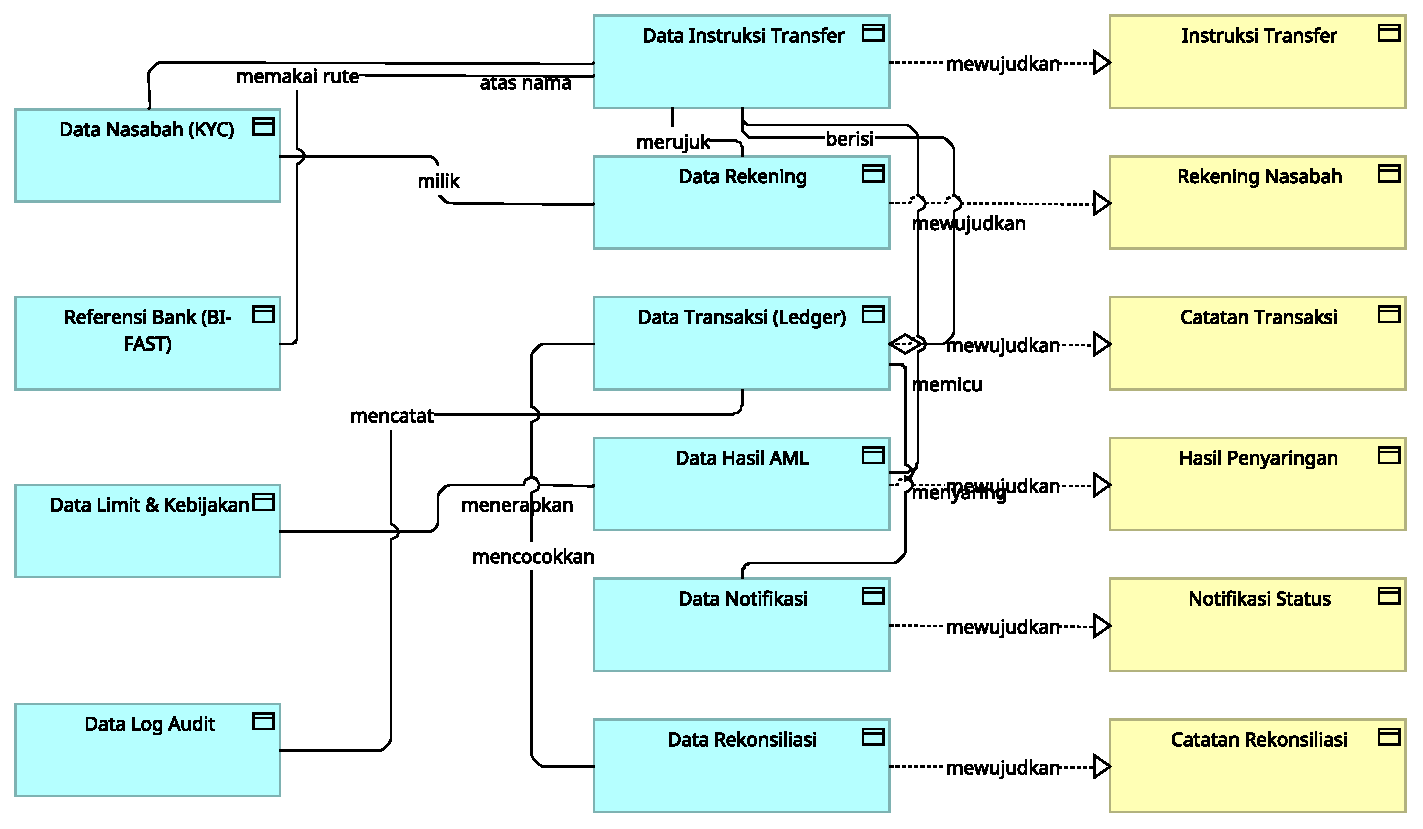
\includegraphics[width=\textwidth,height=.84\textheight,keepaspectratio]{data-transfer.pdf}\\
  {\scriptsize Model data: objek data logis (biru) \emph{merealisasikan} objek
  bisnis konseptual (kuning); data pendukung/master di kiri.}
\end{frame}

\begin{frame}{Cara Membaca Diagram Data}
  \vspace{4pt}
  \footnotesize
  \begin{itemize}\setlength{\itemsep}{2.5pt}
    \item \textbf{Realisasi (kanan):} tiap objek data \emph{mewujudkan} objek
          bisnis di sebelahnya---data diturunkan dari objek bisnis.
    \item \textbf{Model data (tengah/kiri):} Data Transaksi \emph{berisi} Data
          Instruksi; instruksi \emph{merujuk} rekening, \emph{atas nama} nasabah.
    \item \textbf{Data pendukung:} Data Nasabah (KYC), Referensi Bank (BI-FAST),
          Data Limit \& Kebijakan, Data Log Audit.
    \item Tiap garis \emph{berlabel} sehingga model terbaca sebagai kalimat.
  \end{itemize}
  \takeaway{Simpul terpadat = Data Transaksi \& Data Instruksi Transfer: di
  sinilah kualitas dan kunci data paling kritis.}
\end{frame}

\begin{frame}{}
  \centering
  \vspace{1mm}
  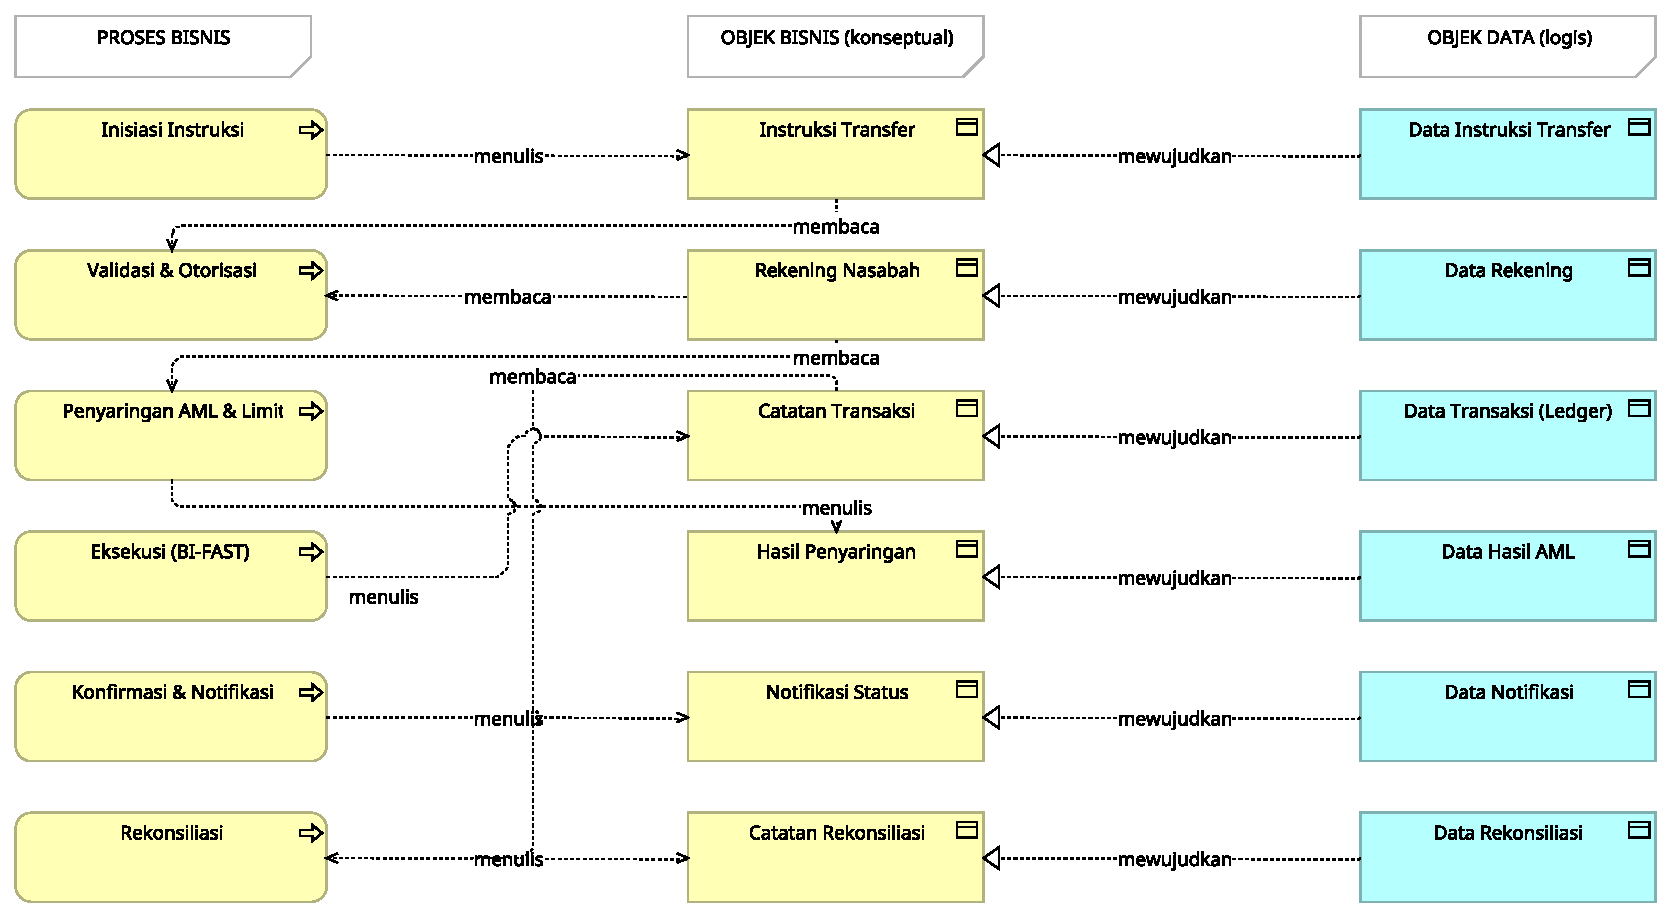
\includegraphics[width=\textwidth,height=.84\textheight,keepaspectratio]{data-akses.pdf}\\
  {\scriptsize Keterlacakan data-ke-proses: proses \emph{mengakses} objek bisnis,
  dan objek data \emph{merealisasikan}-nya (proses tak mengakses data langsung).}
\end{frame}

% ============================================================
\section{Latihan dan Jembatan}
\sectionframe{Latihan dan Jembatan}

\begin{frame}{Latihan Terapan Individual}
  \vspace{8pt}
  \begin{itemize}
    \item \textbf{Latihan 6.1} -- Katalog \& model data (objek data dari objek
          bisnis, relasi berlabel, pemilik/definisi).
    \item \textbf{Latihan 6.2} -- Matriks data-ke-proses (akses baca/tulis).
    \item \textbf{Latihan 6.3} -- Tata kelola \& privasi (sensitivitas, retensi,
          dasar pemrosesan; UU PDP, PP 71).
    \item \textbf{Latihan 6.4} -- Baseline, target, dan paragraf analisis data.
  \end{itemize}
  \takeaway{Semua latihan menjadi bahan langsung Metode dan Analisis domain data
  makalah.}
\end{frame}

\begin{frame}{Jembatan ke Bab Berikutnya}
  \vspace{8pt}
  \begin{itemize}
    \item Bab berikutnya melengkapi Fase C dengan \textbf{lapisan aplikasi}:
          komponen, layanan, antarmuka, dan fungsi aplikasi.
    \item Aplikasi \emph{menjalankan} proses bisnis dan \emph{mengakses} objek
          data yang telah dimodelkan di sini.
    \item Katalog entitas \& matriks data-ke-proses menjadi masukan langsung
          memilih komponen aplikasi dan pola integrasi.
  \end{itemize}
  \takeaway{Model data yang jelas adalah fondasi bagi arsitektur aplikasi dan
  teknologi.}
\end{frame}

\begin{frame}{\hfill}
  \centering
  \Huge{\textbf{Terima kasih}}\\[8pt]
  \normalsize Pertanyaan \& diskusi
\end{frame}

\end{document}
